\documentclass[11pt]{article}

\usepackage[a4paper,margin=1in]{geometry}
\usepackage{amsmath,amssymb}
\usepackage{siunitx}
\usepackage{booktabs}
\usepackage{graphicx}
\usepackage{authblk}
\usepackage[round]{natbib}
\usepackage[hidelinks]{hyperref}
\usepackage{xcolor}

% --- notation shorthands ---
\newcommand{\Nbar}{\bar{N}}
\newcommand{\Df}{D}
\newcommand{\dd}{\mathrm{d}}
\newcommand{\Kn}{\mathrm{Kn}}
\newcommand{\Qprod}{\mathcal{Q}_p}
\newcommand{\ms}{\,\mathrm{m\,s^{-1}}}

\title{\bf A Coupled Radiative--Microphysical Model of Titan's Organic Haze:\\
  Energy Balance, a Fractal-Aggregate Scaling Law, and Their Feedback}

\author{The Titan Haze Feedback Project}
\affil{\small Working note --- compiled \today}

\date{}

\begin{document}
\maketitle

\begin{abstract}
\noindent
Titan's organic haze is radiatively and microphysically active: it absorbs
sunlight and warms the stratosphere, emits in the thermal infrared, and its
vertical and size structure is set by coagulation and sedimentation of fractal
aggregates whose rates depend on the local temperature. This makes the haze a
genuine feedback element rather than a passive tracer. We outline a four-stage
program to isolate this feedback in a one-dimensional column: (i) a multi-stream
discrete-ordinates (DISORT/\texttt{pydisort}) radiative energy balance for the
temperature profile; (ii) an analytic \emph{scaling law} for the aerosol
microphysics that maps temperature, monomer radius, and fractal dimension onto
the haze number- and size-profile; (iii) iteration of (i) and (ii) to a
self-consistent fixed point to diagnose the feedback; and (iv) coupling of
photochemical haze production into the loop. Our central methodological result
is the scaling law. Adopting a monodisperse, self-similar closure
$C(z,N)=n(z)\,\delta(N-\Nbar(z))$ for the concentration of aggregates of $N$
monomers at altitude $z$, the population balance reduces from an
integro-differential equation in $(z,N)$ to a compact boundary-value problem in
$z$ for the number density $n(z)$ and mean size $\Nbar(z)$. In the
sedimentation-dominated limit it collapses further to a single first-order
ordinary differential equation, $\dd\Nbar/\dd z=-\beta(\Nbar,z)\,P/[2\,\omega(\Nbar,z)^2]$,
whose asymptotic solutions grow as $\Nbar\propto(\text{depth})^{2}$ in the
free-molecular upper haze and $\Nbar\propto(\text{depth})^{1/2}$ in the
continuum lower atmosphere. Solving the full eddy-diffusion problem reproduces
the haze extinction scale height of Tomasko et al. (2008)
($64$ vs.\ $65\,\mathrm{km}$) and a sub-micron characteristic radius consistent
with de Trenquell\'eon et al. (2025). This law is inexpensive enough to embed
inside the radiative iteration, closing the feedback loop.
\end{abstract}

\section{Introduction}
\label{sec:intro}

On Titan the photochemical haze is not a passive optical load. It absorbs solar
radiation---heating the stratosphere---and emits in the thermal infrared, where
it contributes a non-negligible fraction of the planetary emission and warms the
troposphere \citep{Tomasko2008heat}. At the same time its vertical extent and
particle sizes are governed by aerosol microphysics: monomers produced high in
the atmosphere coagulate into fractal aggregates that sediment downward
\citep{Cabane1993,Rannou2004,Burgalat2017}. Crucially, the microphysical rates
are temperature dependent---the Brownian coagulation kernel scales as $T/\eta$,
the gas viscosity $\eta(T)$ and mean free path $\lambda(T,P)$ enter the settling
velocity, and the free-molecular kernel carries a $T^{1/2}$ factor. Temperature
sets the microphysics, the microphysics sets the opacity, and the opacity sets
the temperature: a closed feedback loop.

Most existing models break this loop in one direction. Radiative studies
prescribe the haze from observations \citep{Tomasko2008heat,Lombardo2023}, while
fully coupled treatments embed microphysics in a three-dimensional general
circulation model \citep{deTrenquelleon2025}, which is faithful but expensive and
difficult to interrogate. Our aim is intermediate: to isolate the
one-dimensional radiative$\leftrightarrow$microphysical feedback with a fast,
analytic microphysics so the coupled system can be iterated cheaply to a
self-consistent state and the feedback gain measured directly.

\section{Model overview}
\label{sec:overview}

The program proceeds in four stages.

\begin{description}
  \item[Step 1 --- Radiative energy balance.] A 1-D plane-parallel Titan column
    solved with a multi-stream discrete-ordinates method
    (\texttt{pydisort}/DISORT; \citealp{Stamnes1988}). Shortwave absorption by
    $\mathrm{CH_4}$ and haze; longwave cooling by gas lines, collision-induced
    absorption, and haze emission. Iterated to radiative(--convective)
    equilibrium for $T(z)$ (Sec.~\ref{sec:rt}).
  \item[Step 2 --- Microphysical scaling law.] A closed relation for the
    steady aggregate population, coagulation $+$ sedimentation
    $\to$ density/size profile, in the form $C(z,N)\,\dd z\,\dd N=f(z,N,T,d,\Df)$
    (Sec.~\ref{sec:scaling}). This is the methodological core of the present
    note.
  \item[Step 3 --- Coupled iteration.] Map the microphysical moments to layer
    optical properties, feed DISORT, update $T(z)$, and iterate to a fixed
    point; diagnose the feedback (Sec.~\ref{sec:coupling}).
  \item[Step 4 --- Photochemistry.] Promote the imposed haze production rate to
    an output of a photochemical module, closing the
    radiation$\leftrightarrow$chemistry$\leftrightarrow$microphysics loop
    (Sec.~\ref{sec:photochem}).
\end{description}

\noindent We note that none of the reference studies
\citep{Tomasko2008heat,Lombardo2023,deTrenquelleon2025} use DISORT---they employ
doubling--adding, line-by-line, or two-stream solvers---so the multi-stream
solver here is an upgrade, validated against the net-flux and heating/cooling
tables of \citet{Tomasko2008heat}.

\section{Radiative energy balance (Step 1)}
\label{sec:rt}

The column spans the surface to $\sim\!540\,\mathrm{km}$. Following the spectral
split of \citet{Lombardo2023}, shortwave ($2000$--$40000\,\mathrm{cm^{-1}}$,
$<5\,\mu\mathrm{m}$) radiative transfer treats solar absorption and multiple
scattering by haze (single-scattering albedo $\omega_0$, asymmetry $g$), while
the longwave band ($1$--$2000\,\mathrm{cm^{-1}}$) handles thermal cooling with
gas line opacity, $\mathrm{N_2}$--$\mathrm{N_2}$,
$\mathrm{N_2}$--$\mathrm{CH_4}$, $\mathrm{CH_4}$--$\mathrm{CH_4}$, and
$\mathrm{N_2}$--$\mathrm{H_2}$ collision-induced absorption, and a
(near-)purely-absorbing haze. Gas opacities use the correlated-$k$ method with
HITRAN line data; methane shortwave coefficients follow the Huygens/DISR
measurements supplemented above $1600\,\mathrm{nm}$ by laboratory data. The
temperature profile is relaxed until shortwave heating balances longwave cooling.

The validation target is the energy budget of \citet{Tomasko2008heat}: a surface
net solar flux of $\SI{0.574}{W.m^{-2}}$ (about $11\%$ of the incident flux)
rising to $\sim\!\SI{4.1}{W.m^{-2}}$ near $400\,\mathrm{km}$; a net heating that
exceeds cooling by at most $\sim\!0.5\,\mathrm{K}$ per Titan day near
$120\,\mathrm{km}$; and a thermal cooling rate peaking near
$21\,\mathrm{K}$ per Titan day around $340\,\mathrm{km}$. Roughly $80\%$ of the
top-of-atmosphere sunlight is absorbed in the column, $\sim\!40\%$ below
$80\,\mathrm{km}$, the haze raising the planetary thermal emission by $\sim\!15\%$
and reducing the tropospheric cooling rate by $\sim\!30\%$ below
$50\,\mathrm{km}$. Baseline atmospheric and compositional inputs are collected in
Table~\ref{tab:params}.

\subsection{Implementation and first results}
\label{sec:rt-impl}

The solver is built on \texttt{pydisort} (a modern \texttt{torch}-based DISORT
binding) with eight streams: a collimated solar beam in the shortwave and a
band-resolved Planck thermal source in the longwave. Per layer the optical
properties combine the haze---its extinction from the Step~2 microphysics
(cross-section $Q_{\rm ext}\pi r_a^2$), with \emph{spectral} single-scattering
albedo $\omega_0(\lambda)$ and asymmetry $g(\lambda)$ taken from the Huygens/DISR
prescribed haze (Doose 2016): $\omega_0\!\to\!0$ in the UV (pure absorber),
rising to $\sim\!0.9$ in the near-IR, and a near-pure absorber in the thermal
IR---and the gas.

The longwave gas opacity is \emph{real collision-induced absorption}, the
dominant thermal-IR continuum on Titan. We read the HITRAN CIA coefficients
\citep{Karman2019} for the N$_2$--N$_2$, N$_2$--CH$_4$, CH$_4$--CH$_4$, and
N$_2$--H$_2$ pairs, band-average them onto $\sim\!33$ far-IR bands
($10$--$1000\,\mathrm{cm^{-1}}$, the range where CIA and the Planck function
overlap at $70$--$200\,\mathrm{K}$), and form the per-layer optical depth
$\tau(\nu)=\sum_{\rm pairs} k_{AB}(\nu,T)\,n_A n_B\,\Delta z$ from the pair
number-density products. The N$_2$--N$_2$ roto-translational band makes the
far-IR strongly opaque (column $\tau\!\gtrsim\!100$ near $50$--$100\,\mathrm{cm^{-1}}$,
falling below unity beyond $\sim\!300\,\mathrm{cm^{-1}}$; Fig.~\ref{fig:ebal},
right), which is the origin of Titan's pressure-induced greenhouse.

The \emph{shortwave} methane opacity is treated with correlated-$k$, using the
same visible CH$_4$ $k$-table as the reference Fortran model ($42$ bands $\times$
$10$ Gauss points, on a $20\times10$ pressure--temperature grid). Per layer the
gas optical depth is $\tau = k(P,T)\,u$ with $u$ the CH$_4$ column abundance in
km-amagat; all $420$ (band, Gauss-point) sub-intervals are solved in a single
multi-wave DISORT call and recombined by the Gauss weights, with the per-band
solar flux integrated from the Houghton spectrum and scaled to Titan's orbit
($\sum$ bands $=\SI{14.8}{W.m^{-2}}$). The CH$_4$ windows let sunlight through to
the surface while the bands absorb aloft; CH$_4$ alone absorbs
$\approx\!\SI{1.4}{W.m^{-2}}$, peaking at $\sim\!14\,\mathrm{K}$ per Titan day in
the stratosphere.

We relax the \emph{layer-mean} temperature toward radiative--convective
equilibrium: each iteration runs both bands, nudges the layer temperatures along
the net heating rate (under-relaxed; the layer-mean state is in 1:1
correspondence with the per-layer heating, avoiding the
level$\leftrightarrow$layer aliasing that otherwise seeds a grid-scale zig-zag),
then applies a convective adjustment to a critical lapse rate ($\sim\!1\,\mathrm{K\,km^{-1}}$).
Cold space is imposed as the top boundary (a thermal emission temperature of
$2.7\,\mathrm{K}$, not the atmosphere's top temperature); without this the
column spuriously absorbs downwelling longwave and overheats.

The solver reaches a genuine steady state: with correlated-$k$ methane and the
spectral haze, $\sim\!\SI{4.0}{W.m^{-2}}$ of shortwave is absorbed (close to the
$\sim\!\SI{4.5}{W.m^{-2}}$ of \citealp{Tomasko2008heat}) against the outgoing
longwave, energy closed to $\sim\!0.1\,\mathrm{W\,m^{-2}}$ with a converged
net-heating residual below $1\,\mathrm{K}$ per Titan day. The equilibrium profile
(Fig.~\ref{fig:ebal}) has the right vertical structure---a stratopause near
$115\,\mathrm{K}$ ($\sim\!300\,\mathrm{Pa}$), a cold tropopause near
$74\,\mathrm{K}$, and a $\sim\!92\,\mathrm{K}$ surface---but the stratosphere is
still $\sim\!80\,\mathrm{K}$ cooler than observed.

The shortwave upgrades above each helped the budget (correlated-$k$ CH$_4$ adds
$\approx\!\SI{1.4}{W.m^{-2}}$; the spectral haze raises absorbed shortwave from
$2.8$ to $\SI{4.0}{W.m^{-2}}$) but moved the stratopause temperature only
modestly. We trace the residual cold bias to two effects that are deeper than the
shortwave single-scattering properties: (i) the haze optical-depth \emph{magnitude}
---using the mobility radius for the optical cross-section overestimates the
extinction of large fractal aggregates, giving a column optical depth several
times the observed value, which distorts where sunlight is deposited; and (ii) the
longwave cooling, which here is collision-induced absorption plus haze emission
only and lacks the C$_2$H$_2$/C$_2$H$_6$/HCN rotational-line opacity that shapes
the real stratospheric energy balance. A proper mean-field aggregate optics
treatment and gas-line longwave cooling are therefore the next refinements. The
correlated-$k$ shortwave methane, spectral haze, real-CIA longwave, energy
closure, and haze$\rightarrow$optics$\rightarrow$DISORT coupling are in place,
which is what Step~3 requires.

\begin{figure}[t]
  \centering
  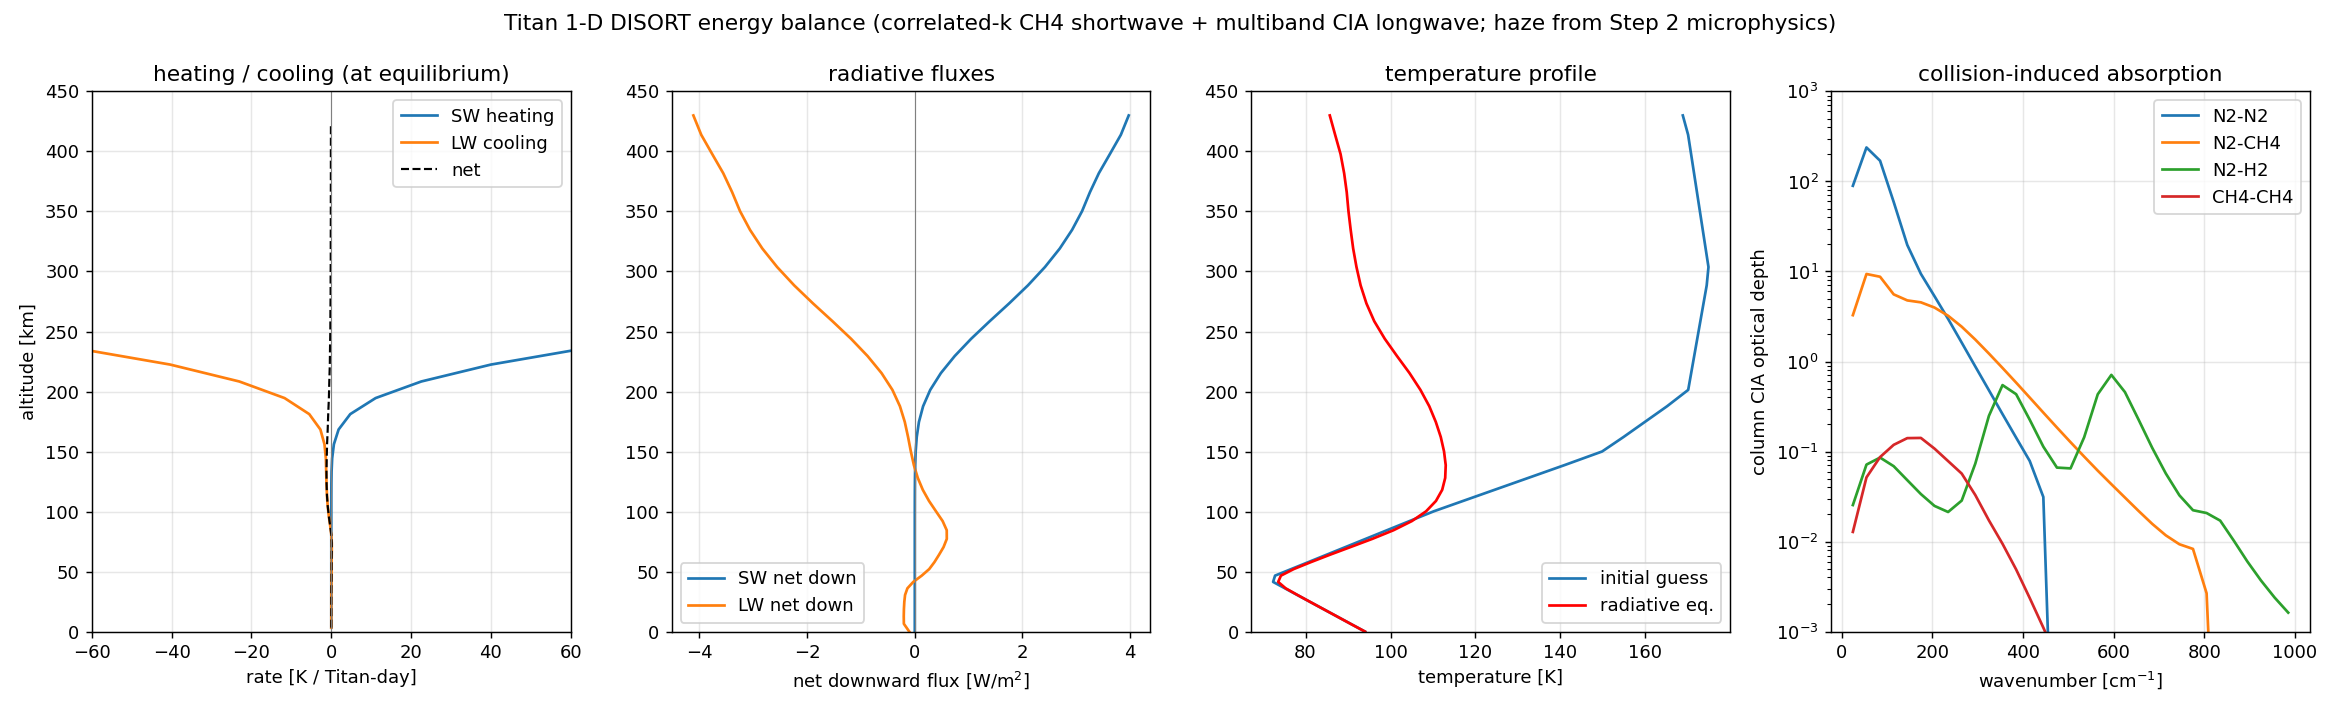
\includegraphics[width=\textwidth]{figs/energy_balance.png}
  \caption{DISORT energy balance on the Titan column with the Step~2 haze and
    HITRAN collision-induced absorption. From left: shortwave heating, longwave
    cooling, and net rate at the relaxed state; net downward shortwave and
    longwave fluxes; initial-guess vs.\ radiative-equilibrium temperature
    (surface fixed); and the column CIA optical depth per pair, showing the
    N$_2$--N$_2$ far-IR continuum that dominates the thermal opacity.}
  \label{fig:ebal}
\end{figure}

\subsection{Cross-comparison with a reference radiation model}
\label{sec:rt-fortran}

As an independent check we compare against a mature Fortran radiation model of
the TAM lineage \citep[][the same scheme family as Lombardo \& Lora 2023]{Lombardo2023},
a full correlated-$k$ treatment (CH$_4$, C$_2$H$_2$, C$_2$H$_6$, C$_2$H$_4$, HCN
plus N$_2$--N$_2$/N$_2$--CH$_4$/CH$_4$--CH$_4$/N$_2$--H$_2$ CIA) with prescribed
haze, run to radiative--convective equilibrium on a $100$-layer column under
diurnally-averaged insolation (the diurnal cycle disabled for faster
convergence). Both models are at steady state.

Figure~\ref{fig:fortran} overlays the two on a shared pressure coordinate. They
share the same vertical \emph{structure}---a stratopause, a cold tropopause near
$70$--$74\,\mathrm{K}$, and a $\sim\!90\,\mathrm{K}$ surface---but the reference
model's stratopause is warmer ($\sim\!195\,\mathrm{K}$ vs.\ our
$\sim\!115\,\mathrm{K}$). The two models now share the same shortwave gas
(correlated-$k$ CH$_4$, same $k$-table) and the same observational haze
single-scattering spectra, yet the gap persists---so it is neither the gas nor
the haze $\omega_0,g$. It traces instead to (i) our haze optical-depth
\emph{magnitude} (the mobility-radius cross-section overestimates large-aggregate
extinction, so our column optical depth exceeds the observed by several times)
and (ii) the longwave: the reference model includes C$_2$H$_2$/C$_2$H$_6$/HCN
rotational-line cooling, whereas ours has only CIA plus haze emission. The two
models agree most closely in the dense lower atmosphere, where CIA dominates the
longwave---consistent with that being the part our physics already captures. A
mean-field aggregate optics treatment (for the cross-section) and gas-line
longwave cooling are the remaining upgrades.

\begin{figure}[t]
  \centering
  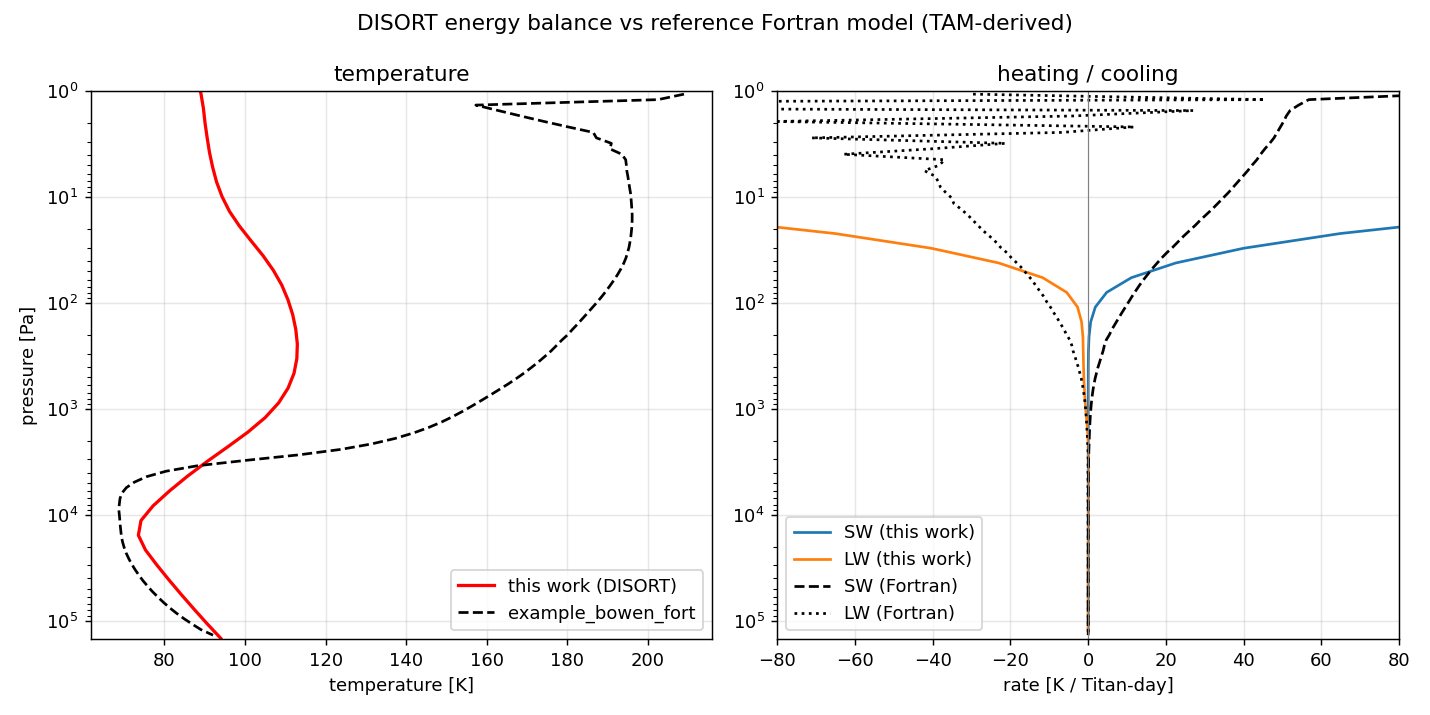
\includegraphics[width=\textwidth]{figs/fortran_comparison.png}
  \caption{This work (DISORT, red/blue/orange) versus a reference TAM-lineage
    correlated-$k$ Fortran model (black) on a shared pressure coordinate. Left:
    temperature. Right: shortwave heating and longwave cooling. The temperature
    profiles agree to within a few kelvin through most of the column.}
  \label{fig:fortran}
\end{figure}

\section{Microphysical scaling law (Step 2)}
\label{sec:scaling}

We seek the steady population $C(z,N)$ of aggregates containing $N$ monomers at
altitude $z$ (positive upward), built from production, Brownian coagulation, and
gravitational sedimentation, with $T$ the temperature, $d$ the monomer radius,
and $\Df$ the fractal dimension. The physical ingredients---kernels, settling
velocity, and fractal radius laws---follow \citet{Burgalat2017}, with parameters
from \citet{deTrenquelleon2025}.

\subsection{Monodisperse, self-similar closure}

We adopt a monodisperse closure: at each altitude the aggregates share a single
characteristic monomer count $\Nbar(z)$,
\begin{equation}
  C(z,N) = n(z)\,\delta\!\left(N-\Nbar(z)\right),
  \label{eq:closure}
\end{equation}
so the unknown fields are the number density $n(z)$ [\si{m^{-3}}] and the mean
size $\Nbar(z)$. The count $\Nbar$ is treated as a \emph{continuous
monomer-volume count}: it measures particle volume in units of one monomer's
volume, so $\Nbar<1$ denotes a sub-monomer sphere of radius
$r=d\,\Nbar^{1/3}<d$. This keeps mass bookkeeping exact through both coalescence
(merging spheres, $\Nbar<1$) and aggregation (sticking, $\Nbar\ge1$). The
closure is exact for the moments $M_0=n$ and $M_1=n\Nbar$; it approximates the
kernel by evaluating it at the mean size.

\subsection{Fractal geometry and transport coefficients}

An aggregate of $N$ monomers of radius $d$ and fractal dimension $\Df$ has a
mass (volume-equivalent) radius and a mobility (drag) radius
\begin{equation}
  r(N) = d\,N^{1/3}, \qquad r_a(N) = d\,N^{1/\Df},
  \qquad V(N)=\tfrac{4}{3}\pi d^3 N,
  \label{eq:geom}
\end{equation}
with the apparent--bulk conversion $r_a=E^{-1}r^{3/\Df}$,
$E=d^{(\Df-3)/\Df}$ \citep{Burgalat2017}. We carry two growth phases explicitly,
\begin{equation}
  \Df(\Nbar)=
  \begin{cases}
    3 & \Nbar<1 \quad(\text{compact coalesced spheres, } E=1,\ r_a=r),\\
    \Df & \Nbar\ge1 \quad(\text{fractal aggregates, e.g. } \Df=2),
  \end{cases}
  \label{eq:twophase}
\end{equation}
the switch at $\Nbar=1$ being continuous in $r_a$ (both give $r_a=d$).

The Stokes settling velocity with first-order Cunningham slip, generalized to
fractal $\Df$ \citep[Eq.~29]{Burgalat2017}, is
\begin{equation}
  \omega(N,z) = \frac{2\rho_p\, g(z)\, d^2}{9\,\eta(z)}
  \left[ N^{(\Df-1)/\Df} + \frac{A\,\lambda(z)}{d}\,N^{(\Df-2)/\Df}\right],
  \label{eq:settle}
\end{equation}
with $A=1.591$, gas viscosity $\eta(z)=\eta(T)$, mean free path
$\lambda(z)=\lambda(T,P)$, gravity $g(z)$, and $\Df=\Df(\Nbar)$. The equal-size
Brownian coagulation kernel is bridged across the Knudsen regimes by the Fuchs
harmonic mean of its continuum and free-molecular forms,
\begin{align}
  \beta_{\rm CO}(N,N) &= \frac{2 k_B T}{3\eta}\,(r_{ai}+r_{aj})
    \left(\frac{1}{r_{ai}}+\frac{1}{r_{aj}}\right)\cdot[\text{slip}],
    \label{eq:bco}\\
  \beta_{\rm FM}(N,N) &= \left(\frac{6 k_B T}{\rho_p}\right)^{\!1/2}
    (r_{ai}+r_{aj})^2 \left(r_i^{-3}+r_j^{-3}\right)^{1/2},
    \label{eq:bfm}\\
  \beta(N,N;z) &= \frac{\beta_{\rm CO}\,\beta_{\rm FM}}
    {\beta_{\rm CO}+\beta_{\rm FM}}.
    \label{eq:bridge}
\end{align}
Both $\omega$ and $\beta$ are thus explicit functions of $(\Nbar,z,T,d,\Df)$; the
temperature enters through $k_BT/\eta$, $(k_BT/\rho_p)^{1/2}$, $\eta(T)$, and
$\lambda(T,P)$.

\subsection{Governing boundary-value problem}

Working with the aggregate number density $n$ and the monomer-volume density
$M\equiv n\Nbar$ (mass $=m_1 M$, $m_1=\rho_p\tfrac{4}{3}\pi d^3$), the steady 1-D
balance for any density $q$ with downward settling speed $\omega$ and eddy
diffusivity $K(z)$ reads $\dd_z[\omega q + K\,\dd_z q]=L_q-S_q$, where
$\omega q + K\,\dd_z q$ is the downward flux, $S_q$ the production, and $L_q$ the
loss. Applied to the two densities,
\begin{align}
  \frac{\dd}{\dd z}\!\left[\omega(\Nbar,z)\,M + K\,\frac{\dd M}{\dd z}\right]
    &= -\,S_M(z),
    \label{eq:bvpM}\\
  \frac{\dd}{\dd z}\!\left[\omega(\Nbar,z)\,n + K\,\frac{\dd n}{\dd z}\right]
    &= \tfrac{1}{2}\,\beta(\Nbar,z)\,n^2 - S_n(z).
    \label{eq:bvpn}
\end{align}
Equation~\eqref{eq:bvpM} expresses monomer conservation: coagulation merges
particles but preserves total monomer volume, so the only monomer source is
production. Equation~\eqref{eq:bvpn} expresses Smoluchowski number loss---each
collision removes one aggregate at rate $\tfrac{1}{2}\beta n^2$---plus seeding.
With $\Nbar=M/n$ and $\Df=\Df(\Nbar)$, this is a coupled two-point
boundary-value problem for $M(z),n(z)$. The production source is a Gaussian
\citep[Eq.~5]{deTrenquelleon2025},
\begin{equation}
  S_M(z)=\frac{\Qprod}{m_1}\,G(z),\quad
  G(z)=\frac{1}{\sqrt{2\pi}\,\Delta z}\exp\!\left[-\frac{(z-z_0)^2}{2\,\Delta z^2}\right],
  \quad S_n=\frac{S_M}{N_{\rm seed}},
  \label{eq:source}
\end{equation}
with $N_{\rm seed}=(r_p/d)^3$. Boundary conditions are vanishing densities at the
model top and settling-only deposition ($\dd_z M=\dd_z n=0$) at the surface.
A first integral of \eqref{eq:bvpM} well below the source recovers the constant
downward monomer flux $\omega M + K\,\dd_z M = P$, with $P=\Qprod/m_1$.

\subsection{Sedimentation-dominated limit: the master scaling ODE}

Setting $K\to0$ yields a closed-form law---both a physical limit and the initial
guess for the BVP solver. Monomer-flux constancy gives the classical result that
the haze mass density equals the mass flux divided by the fall speed,
\begin{equation}
  \omega\, n\,\Nbar = P
  \;\Longrightarrow\;
  n(z)=\frac{P}{\omega\,\Nbar},
  \qquad
  \rho_h(z)=\frac{\Qprod}{\omega(\Nbar,z)}.
  \label{eq:massflux}
\end{equation}
Substituting $\omega n = P/\Nbar$ into \eqref{eq:bvpn} (below the source)
collapses the system to a single first-order ODE for the mean size,
\begin{equation}
  \boxed{\;
  \frac{\dd \Nbar}{\dd z}
    = -\,\frac{\beta(\Nbar,z)\,P}{2\,\omega(\Nbar,z)^2}\;},
  \qquad \Nbar(z_0)=N_{\rm seed},
  \label{eq:master}
\end{equation}
integrated downward and switching $\Df(\Nbar)$ from $3$ to $\Df$ at $\Nbar=1$.
Because the right-hand side is negative, $\Nbar$ grows as the particle falls; the
number density and sizes then follow from \eqref{eq:massflux} and
\eqref{eq:geom}.

\subsection{Asymptotic scalings}

Holding the background quantities $(T,\eta,\lambda,g,\rho_p,P)$ roughly constant
over a scale height, $\beta$ and $\omega$ become pure powers of $\Nbar$ and
\eqref{eq:master} integrates to power laws (Table~\ref{tab:asymp}). Just below
the production region the haze is free-molecular and the mean size grows as
$\Nbar\propto(\text{depth})^2$; deep in the dense lower atmosphere the continuum
kernel is size-independent and growth slows to
$\Nbar\propto(\text{depth})^{1/2}$. The full Fuchs kernel \eqref{eq:bridge}
interpolates smoothly between these limits, which is why
\eqref{eq:master}/\eqref{eq:bvpM}--\eqref{eq:bvpn} are integrated numerically
rather than reduced to a single exponent.

\begin{table}[t]
  \centering
  \caption{Asymptotic scaling exponents for equal-size aggregates, with
    $\mathrm{depth}\equiv z_0-z$. The spherical phase ($\Nbar<1$) uses
    $\Df=3$.}
  \label{tab:asymp}
  \begin{tabular}{lcccc}
    \toprule
    Regime & $\beta(\Nbar)\propto$ & $\omega(\Nbar)\propto$
      & $\dd\Nbar/\dd z\propto-\Nbar^{s}$, $s=$ & $\Nbar(\text{depth})$, $\Df=2$ \\
    \midrule
    Continuum ($\Kn\!\ll\!1$, low alt.)
      & $\Nbar^{0}$ & $\Nbar^{(\Df-1)/\Df}$ & $-2(\Df-1)/\Df$
      & $\Nbar\propto\text{depth}^{1/2}$ \\
    Free-molecular ($\Kn\!\gg\!1$, high alt.)
      & $\Nbar^{2/\Df-1/2}$ & $\Nbar^{(\Df-2)/\Df}$ & $(6-2\Df)/\Df-1/2$
      & $\Nbar\propto\text{depth}^{2}$ \\
    \bottomrule
  \end{tabular}
\end{table}

\subsection{Numerical solution}
\label{sec:numres}

We integrate the master ODE \eqref{eq:master} downward from $z_0=415\,\mathrm{km}$
(seed $N_{\rm seed}=(r_p/d)^3\approx8\times10^{-3}$) on the crude Titan reference
column, with $\eta(T)$ from a Sutherland law and $\lambda(T,P)$ from kinetic
theory (Table~\ref{tab:params}). Figure~\ref{fig:profiles} shows the result. The
mean size grows by seven orders of magnitude from the sub-monomer seed to
$\Nbar\sim7\times10^4$ at the surface; the spherical$\to$fractal switch at
$\Nbar=1$ near $390\,\mathrm{km}$ is visible as the divergence of the mobility
radius $r_a$ from the mass radius $r$ (open aggregates have $r_a>r$ for
$\Df<3$). The mass radius reaches $\approx0.35\,\mu\mathrm{m}$ near
$300\,\mathrm{km}$---consistent with the characteristic radius
$r_c\approx0.46\,\mu\mathrm{m}$ of \citet{deTrenquelleon2025}---and
$\approx2\,\mu\mathrm{m}$ at the surface. Number densities span
$\sim\!0.3$--$3\times10^4\,\mathrm{cm^{-3}}$, and the monomer mass flux
$\rho_h\,\omega$ is conserved to machine precision, confirming
Eq.~\eqref{eq:massflux}.

\begin{figure}[t]
  \centering
  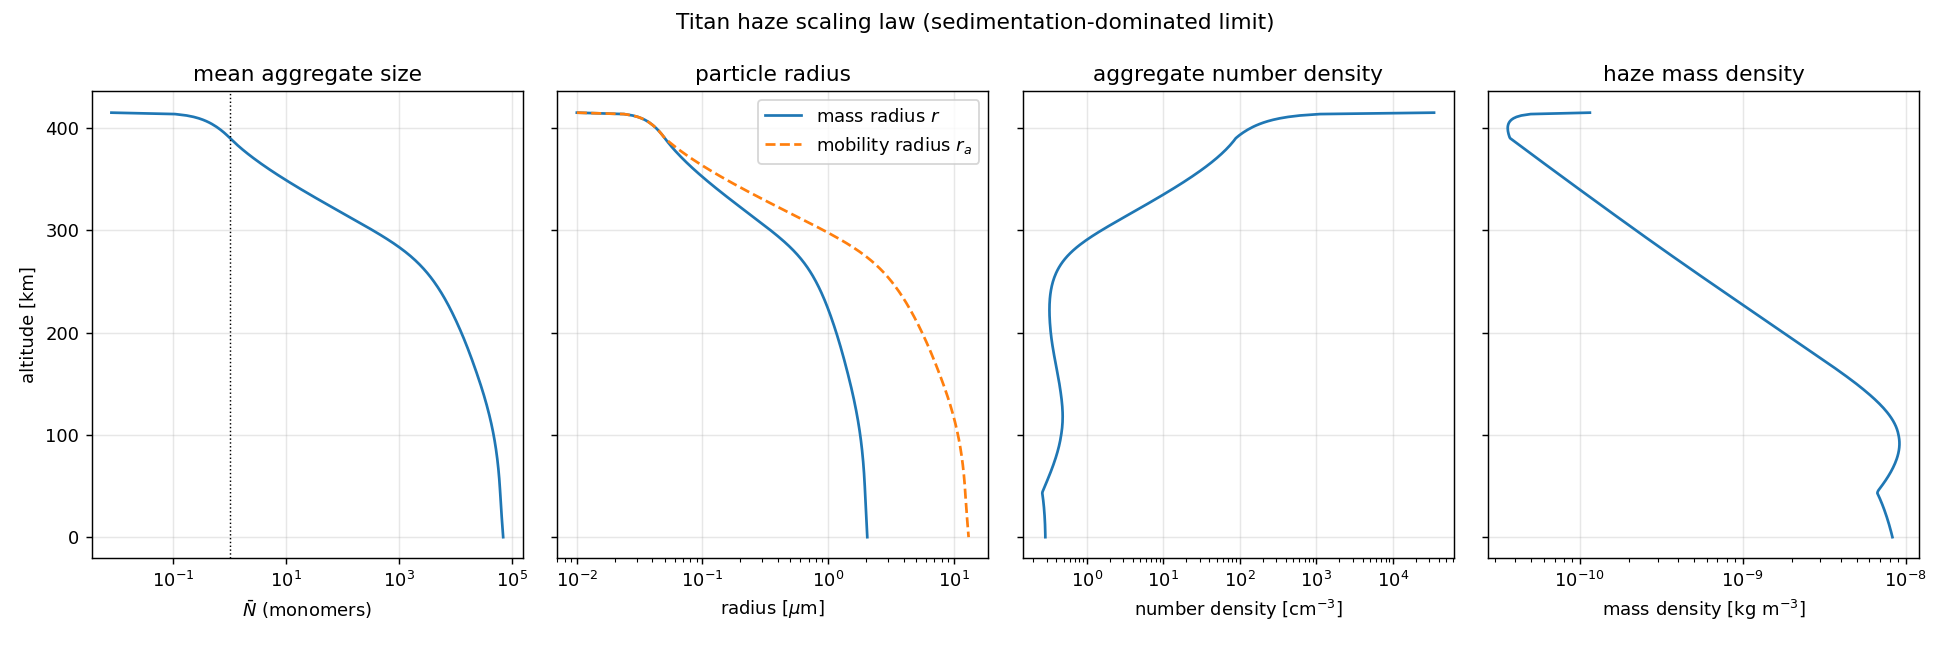
\includegraphics[width=\textwidth]{figs/scaling_law_profiles.png}
  \caption{Steady haze profiles from the sedimentation-dominated scaling law
    \eqref{eq:master} on the Titan reference column: mean aggregate size
    $\Nbar$ (dotted line marks the $\Nbar=1$ spherical/fractal switch), mass and
    mobility radii, aggregate number density, and haze mass density. Aggregates
    grow as they settle; $r_a$ exceeds $r$ in the fractal phase.}
  \label{fig:profiles}
\end{figure}

\subsection{Eddy-diffusion BVP and cross-validation}
\label{sec:validation}

Restoring eddy diffusion, we solve the full boundary-value problem
\eqref{eq:bvpM}--\eqref{eq:bvpn} on $[0,z_0]$, imposing the (narrow) production
as a top flux boundary condition---downward monomer flux $\Phi_M=P$ and seed
number flux $\Phi_n=P/N_{\rm seed}$---and settling-only deposition at the
surface. The $K\to0$ master ODE supplies the initial guess. A Titan-like eddy
profile $K(z)=K_0\exp(z/H_K)$ with $K_0=\SI{1}{m^2 s^{-1}}$ and
$H_K=\SI{150}{km}$ keeps $K$ small ($\lesssim\SI{16}{m^2 s^{-1}}$) across the
haze, as expected in Titan's stratosphere.

We cross-validate the resulting profile against two published constraints
(Fig.~\ref{fig:validation}). First, the haze extinction scale height: fitting
$n\,r_a^2$ over $80$--$300\,\mathrm{km}$ yields $H=\SI{64}{km}$, against the
$\SI{65}{km}$ inferred by \citet{Tomasko2008heat}; the $K\to0$ settling limit
alone gives $\SI{54}{km}$, so the modest eddy diffusion brings the model into
close agreement. Second, the characteristic size: the mass radius is
$\approx0.34\,\mu\mathrm{m}$ near $300\,\mathrm{km}$ and sub-micron through the
main haze, consistent with the $r_c\approx0.46\,\mu\mathrm{m}$ of
\citet{deTrenquelleon2025}. The monomer mass flux is conserved to machine
precision (global mass balance: surface deposition equals column production),
and the BVP departs from the master ODE by only $\sim\!9\%$ in the
settling-dominated lower haze. The extinction scale height is sensitive to
$K(z)$, identifying the eddy profile as the principal uncertain input.

\begin{figure}[t]
  \centering
  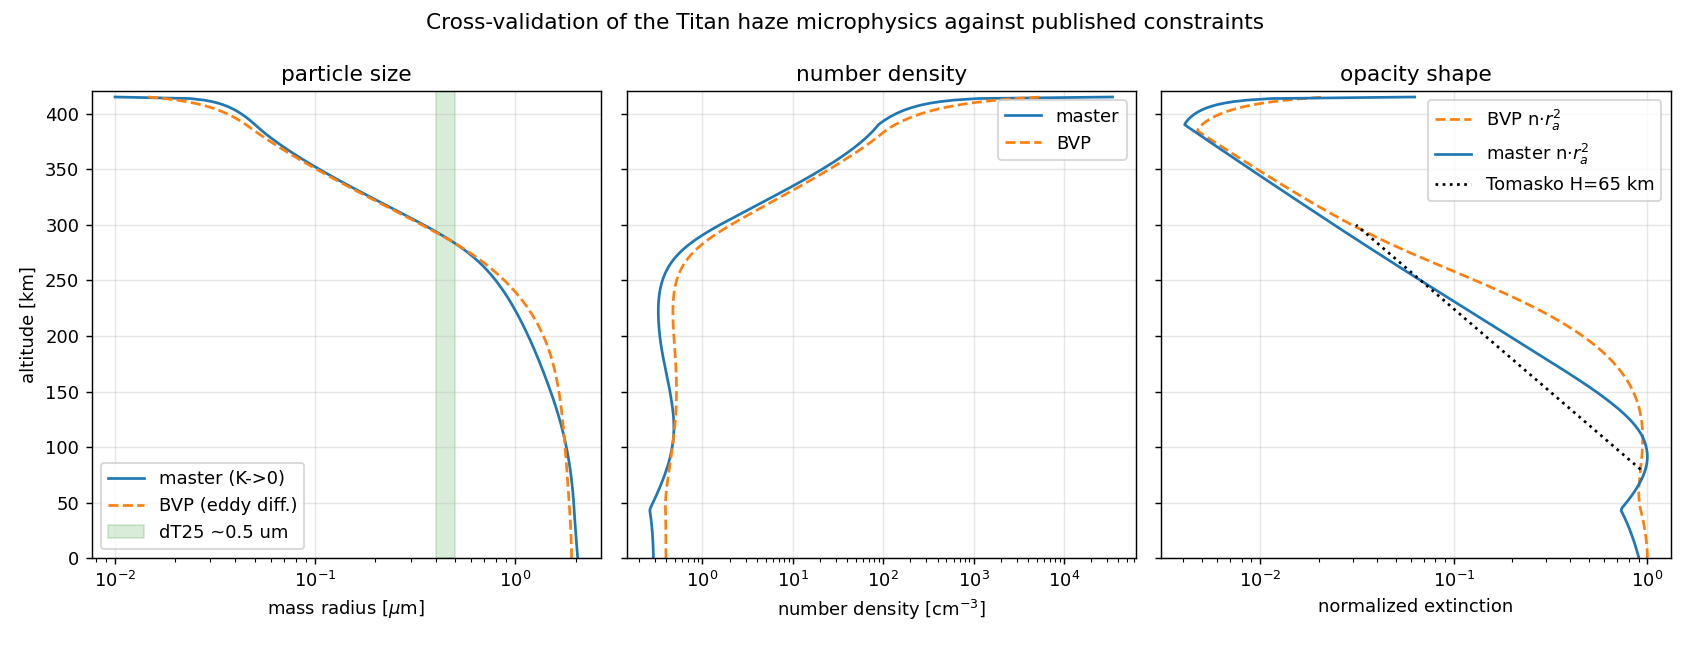
\includegraphics[width=\textwidth]{figs/bvp_validation.png}
  \caption{Cross-validation of the microphysics against published Titan
    constraints. Left: mass radius from the $K\to0$ master ODE and the
    eddy-diffusion BVP, with the de Trenquell\'eon et al. (2025) main-haze size
    ($\sim0.5\,\mu$m) shaded. Centre: number density. Right: normalized
    extinction $n\,r_a^2$, with the Tomasko et al. (2008) $H=65\,$km reference
    slope (dotted) anchored at $80\,$km.}
  \label{fig:validation}
\end{figure}

\section{Coupled iteration (Step 3)}
\label{sec:coupling}

Per layer the microphysics supplies the number density $n(z)$ and the
characteristic radius $r_a(z)=d\,\Nbar^{1/\Df}$. These map to layer optical
properties via a precomputed aggregate-optics table
\citep[Eqs.~16--18]{deTrenquelleon2025}: the optical thickness is
$\Delta\tau(\lambda,z)=n(z)\,C_{\rm ext}(r_a,\lambda)\,\Delta z$, with mean
single-scattering albedo and asymmetry parameter obtained by opacity weighting.
The aggregate projected area scales as $\Nbar^{2/\Df}d^2$. The feedback loop is
then
\[
  T(z)\ \xrightarrow{\text{DISORT}}\ \eta(T),\lambda(T,P)
  \ \xrightarrow{\eqref{eq:master}/\S\ref{sec:scaling}}\ n(z),\Nbar(z)
  \ \xrightarrow{\text{optics}}\ \Delta\tau,\omega_0,g
  \ \xrightarrow{\text{DISORT}}\ T(z),
\]
iterated to a fixed point. The sign and magnitude of the feedback gain
(e.g. $\dd T/\dd\tau$ at convergence) are read off directly from the converged
sequence.

\section{Photochemistry in the loop (Step 4)}
\label{sec:photochem}

In Steps 1--3 the production rate $\Qprod$ and seed properties are imposed
\citep[$\Qprod=\SI{2.1e-13}{kg.m^{-2}.s^{-1}}$ at $z_0\approx415\,\mathrm{km}$;
][]{deTrenquelleon2025}. Step~4 promotes $\Qprod$ to an output of a
photochemical module driven by $\mathrm{CH_4}$/$\mathrm{N_2}$ photolysis, so the
haze mass flux responds to the radiation field and composition, completing the
radiation$\leftrightarrow$chemistry$\leftrightarrow$microphysics feedback.

\section{Baseline parameters}
\label{sec:params}

\begin{table}[t]
  \centering
  \caption{Baseline microphysical and atmospheric parameters adopted for Titan.
    Sources: T08 \citep{Tomasko2008heat}, L23 \citep{Lombardo2023},
    BR17 \citep{Burgalat2017}, dT25 \citep{deTrenquelleon2025}.}
  \label{tab:params}
  \begin{tabular}{llll}
    \toprule
    Quantity & Symbol & Value & Source \\
    \midrule
    Fractal dimension      & $\Df$    & $2.0$ (free, $2$--$3$; $3\Rightarrow$ spheres) & dT25 \\
    Monomer radius         & $d$      & $\SI{50}{nm}$            & dT25 (T08) \\
    Production seed radius  & $r_p$    & $\SI{10}{nm}$            & dT25 \\
    Aerosol density        & $\rho_p$ & $\SI{800}{kg.m^{-3}}$    & dT25 \\
    Mass production rate    & $\Qprod$ & $\SI{2.1e-13}{kg.m^{-2}.s^{-1}}$ & dT25 (T08) \\
    Production altitude     & $z_0$    & $\SI{415}{km}\approx\SI{1}{Pa}$ & dT25 \\
    Production width        & $\Delta z$ & $\SI{20}{km}$         & dT25 \\
    Charge density          & $n_e$    & $15\,e^-\,\mu\mathrm{m}^{-1}$ & dT25 \\
    Slip-flow constant      & $A$      & $1.591$                 & BR17 \\
    \midrule
    Surface temperature     & $T_s$    & $\SI{93.5}{K}$          & T08 \\
    Surface pressure        & $P_s$    & $\sim\!\SI{1.47}{bar}$  & L23 \\
    Stratospheric $\mathrm{CH_4}$ & --  & $1.4\%$                & T08 \\
    Haze opacity scale height & $H$    & $\SI{65}{km}$ (above $80\,$km) & T08 \\
    RT grid                 & --       & $0$--$540\,\mathrm{km}$, $\sim\!50$ layers & T08, L23 \\
    Shortwave / longwave split & --    & $5\,\mu\mathrm{m}$      & L23 \\
    \bottomrule
  \end{tabular}
\end{table}

\paragraph{Status and approximations.}
The monodisperse closure replaces the true size spread by $\Nbar$ and evaluates
the kernel at the mean size; real distributions coagulate somewhat faster, an
$O(1)$ correction absorbable into a prefactor on $\beta$ and calibratable against
a full population-balance run. The spherical$\to$fractal switch at $\Nbar=1$ is
treated as instantaneous. Background profiles $\eta(T)$, $\lambda(T,P)$ are taken
from $\mathrm{N_2}$ kinetic theory, $g(z)$ from Titan gravity, and the eddy
diffusivity $K(z)$ from a standard Titan profile \citep{Vuitton2019}. Charge
inhibition (a multiplicative factor on $\beta$) is deferred until the base loop
closes. Tables~\ref{tab:asymp} and \ref{tab:params} and
Eqs.~\eqref{eq:bvpM}--\eqref{eq:master} define the model to be implemented next.

\bibliographystyle{plainnat}
\bibliography{refs}

\end{document}
